\chapter{Medidas Diretas e Indiretas}
\label{sec:medidasDir&Indir}
\vspace{-0.5cm}
Para estabelecer o valor de uma grandeza temos que utilizar um instrumento de medi\c c\~ao e um m\'etodo de medi\c c\~ao. Al\'em disso, ser\'a necess\'ario definir as unidades em que essa magnitude \'e medida. Por exemplo, se queremos medir a largura de uma mesa, utilizaremos uma r\'egua e, dependendo do sistema de medi\c c\~ao escolhido, expressaremos o valor medido em unidades de comprimento como, por exemplo, o metro (m) para o sistema de unidades internacional (SI) ou centmetros (cm) no caso do CGS. O m \'etodo de medi\c c\~ao consistir\'a em determinar a quantidade de unidades da menor fra\c c\~ao da r\'egua que correspondem ao comprimento que se deseja medir. Quando uma medi\c c\~ao  \'e realizada lendo o resultado diretamente em um instrumento (constru\'ido para isso), dizemos que a {\bf medida \'e direta}. H\'a grandezas que n\~ao se medem diretamente, mas que s\~ao obtidas a partir de outras grandezas medidas de forma direta.  Por exemplo, para conhecer \'area de um ret\^angulo medem-se os comprimentos de seus lados ou para determinar o volume de uma esfera deve-se medir o di\^ametro.  Neste caso a {\bf medida \'e indireta}. 
% \'i
%\~ao
%\c c\~oes
\section*{Medidas diretas com flutua\c c\~oes aleat\'orias}\label{stat}

Consideremos uma grandeza da qual se fazem $N$ medi\c c\~oes diretas, que chamaremos: $x_1, x_2, x_3, ... , x_N$. Estes valores ser\~ao geralmente distintos entre si, mas alguns valores podem se repetir. 

Evidentemente n\~ao ser\'a satisfat\'orio fornecer como resultado da medi\c c\~ao uma tabela de $N$ valores. \'E necess\'ario caracterizar a s\'erie de medi\c c\~oes mediante uns poucos par\^ametros que tenham um significado preciso relacionado com a magnitude medida e/ou o processo de medi\c c\~ao utilizado. Os par\^ametros importantes s\~ao:

\begin{enumerate}
\item {\bf Valor m\'edio} \'e  a m\'edia aritm\'etica dos valores medidos
\begin{equation}
\bar{x} = \frac{1}{N} \sum_{i = 1}^N {x_i},
\label{eq:vm}
\end{equation}
\noindent
e é o valor atribu\'ido \`a magnitude medida. É bastante intuitivo considerar a m\'edia aritm\'etica como valor representativo da grandeza medida. A m\'edia aritm\'etica se caracteriza por apresentar as medições ao seu redor, de modo que a soma dos desvios 
\begin{equation}
\delta_i = x_i - \bar{x} ,
\end{equation}
\noindent
é igual a zero. Ou seja,
\begin{equation}
S = \sum_{i=1}^N \delta_i = 0.
\end{equation}

Isto pode ser facilmente demonstrado, escrevendo:
\begin{equation}
S = \sum_{i=1}^N \delta_i =  \sum_{i=1}^N (x_i - \bar{x}),
\end{equation}
\noindent
e distribuindo o somatório, de modo que:
\begin{equation}
S = \sum_{i=1}^N x_i - \sum_{i=1}^N \bar{x}  =  \sum_{i=1}^N x_i - N\bar{x}.
\end{equation}

Utilizando a expressão do valor médio (equação~\ref{eq:vm}):
\begin{equation}
\sum_{i=1}^N x_i = N\bar{x},
\end{equation}
\noindent
obtemos $S = 0$ como queríamos mostrar.

Por esta razão, a soma dos desvios não é um parâmetro que possa ser utilizado para caracterizar a distribuição das medições ao redor do valor médio e é necessário utilizar outro parâmetro.

\item Dispersão das medições ou {\bf desvio padrão} define-se como:
\begin{equation}
\sigma = \sqrt{\frac{\sum_{i=1}^N (x_i - \bar{x})^2}{N-1}}.
\end{equation}
\noindent

O desvio padrão é um parâmetro que caracteriza o processo de medida. Quando as medições são poucas, $\sigma$ pode flutuar, mas para muitas medidas ($N$ grande) estabiliza-se e não depende do número de medições.

\item O {\bf erro ou incerteza do valor médio} é definido como:

\begin{equation}
\xi=\sqrt{\sigma_{m}^2 + \sigma_{r}^2},
\end{equation}

\noindent
onde $\sigma_{m}$ está associado às flutuacões estatísticas em torno do valor médio:

\begin{equation}
\sigma_{m}=\frac{\sigma}{\sqrt{N}},
\end{equation}

\noindent
e $\sigma_{r}$ expressa os erros sistemáticos residuais (por exemplo devido à um instrumento mal calibrado).

Vamos supor que nas nossas medidas não ocorrem tais erros sistemáticos, de forma que usaremos sempre:

\begin{equation}
\xi=\frac{\sigma}{\sqrt{N}},
\end{equation}


O erro do valor médio é a dispersão esperada para as médias de várias séries de medições realizadas nas mesmas condições. O erro do valor médio depende do número de medições como se pode ver na sua expressão, sendo que ela diminui com o aumento do número de medições.



\end{enumerate}

\section*{Medidas Indiretas}\label{prop}

Como j\'a foi definido anteriormente, h\'a grandezas que não podem ser determinadas diretamente, mas que se obt\'em a partir de outras grandezas que, estas sim, são medidas de forma direta. Portanto, as incertezas das grandezas que se medem diretamente devem ser propagadas para contribuir à incerteza da grandeza que se calcula utilizando uma determinada expressão.

Sejam $x_1, x_2, ... , x_N$ grandezas independentes medidas de forma direta, e seja a grandeza que se quer determinar $F = F (x_1, x_2, ..., x_N)$ uma função das grandezas $x_1, x_2, ... , x_N$, cujas incertezas estão dadas por $\delta{x_1}, \delta{x_2}, ... , \delta{x_N}$. Pode-se mostrar que a incerteza de $F$ é dada por: 
\begin{equation}
(\delta F)^2 = \left(\frac{\partial F}{\partial x_1}\right)^2 \cdot \delta{x_1}^2  +  \left(\frac{\partial F}{\partial x_2}\right)^2 \cdot \delta{x_2}^2 + ... +  \left(\frac{\partial F}{\partial x_N}\right)^2 \cdot \delta{x_N}^2,  
\end{equation}
\noindent
ou
\begin{equation}\label{eq:propag-geral}
(\delta F)^2 = \sum_{i = 1}^N \left(\frac{\partial F}{\partial x_i}\right)^2 \cdot \delta{x_i}^2 .
\end{equation}
Esta equação é a f\'ormula de propagação da incerteza para uma grandeza determinada indiretamente.%, ler capítulo 8 do livro de Vuolo para ver a demonstração de esta fórmula.

\section*{Compara\c c\~ao entre duas medidas da mesma grandeza}
Muitas vezes comparamos diferentes resultados experimentais para a medida de uma mesma grandeza.  Estes resultados podem vir por exemplo das diferentes técnicas utilizadas para determinar uma grandeza, ou podem vir de valores conhecidos tabulados na literatura. Vamos supor que temos dois resultados para uma mesma grandeza sendo o primeiro $x_1 \pm \delta{x_1}$ e o segundo $x_2 \pm \delta{x_2}$.  Se eles são estimativas de uma mesma grandeza, esperamos que a discrepância entre eles ($|x_1-x_2|$) seja compatível com zero. Como cada uma das medidas está sujeita a uma flutuação estatística de acordo com sua incerteza, em geral encontramos valores diferentes de zero para a discrepância. Como podemos avaliar se a discrepância é significativamente diferente de zero ?  Há várias formas de se fazer essa avaliação, dependendo do grau de confiança que queremos ter na afirmação de que a diferença é incompatível com zero (ou equivalentemente de que os dois valores são incompatíveis entre si) . Vamos considerar a discrepância entre os valores ($|x_1-x_2|$) pouco significativa ou irrelevante quando for menor que 3 vezes a incerteza da discrepância. Utilizando a expressão para propagação de incertezas definida na Seção~\ref{prop}, determinamos a incerteza da discrepância $\delta |x_1-x_2|=\sqrt{\delta x^2_1+\delta x^2_2}$. Resumindo, duas medidas independentes $x_1$ e $x_2$ da mesma grandeza são consideradas {\bf  compatíveis} quando : 
$$|x_1 - x_2| < 3 \sqrt{\delta x^2_1+\delta x^2_2}$$ 
ou
$$\frac{|x_1 - x_2|}{\sqrt{\delta x^2_1+\delta x^2_2}}<3.$$

Ao contrário, consideramos as duas medidas $x_1$ e $x_2$ {\bf incompatíveis} quando a discrepância entre elas é maior que 3 vezes a incerteza da discrepância. 

 Considere por exemplo a medida de um comprimento de uma mesa cujo resultado é L$_{exp}$=(98~$\pm$~1)~cm. Como podemos ver se esse resultado é compatível com o valor nominal fornecido pelo fabricante, que é de L$_{nom}$=1 m ? 
Como o valor nominal nesse caso não tem incerteza, a incerteza  da discrepância é igual à incerteza da medida experimental. A discrepância é de 2 cm, que é apenas duas vezes a incerteza da discrepância e a medida é, portanto, compatível com o valor nominal. Uma outra forma de ver isso \'e analisando se o valor nominal est\'a contido no intervalo de valores $I_{exp}$=[L-3$\delta L$, L+3$\delta$L]. Nesse caso, o valor 100 cm est\'a contido no intervalo $I_{exp}$=[95,101] cm.

Em um outro exemplo, um estudante mede o valor da aceleração da gravidade e encontra $g_{exp}=9,21\,\pm\,0,01$ m/s$^2$ e quer comparar com o valor tabelado $g=9,787\,\pm\,0,001$ m/s$^2$. Temos:
$$\frac{|g_{exp} -g |}{\sqrt{\delta g^2_{exp}+\delta g^2}}=\frac{0,577}{0,01005}\approx 57\gg 3.$$
Logo, os dois valores são incompat\'iveis.



\section*{Exercícios}

\begin{num}

\item Os lados de um paralelepípedo são $a$ = (4,50 $\pm$ 0,05) cm, $b$ = (8,50 $\pm$ 0,09)~cm e $c$ = (35,0 $\pm$ 0,3) mm. Determinar o volume do cubo com sua incerteza absoluta e relativa.

\item Na medição da resistência (R), se obteve o valor da tensão V = (15,2 $\pm$ 0,2)~V e da corrente I = (2,6 $\pm$ 0,1)~A. Qual é a incerteza absoluta da resistência usando a equação R = V/I?
 
\item Um pêndulo simples é utilizado para medir o valor da aceleração da gravidade utilizando equação:

\[ 
T = 2 \pi \sqrt{\frac{l}{g}}.
\]
\noindent
O período $T$ medido foi de (1,24 $\pm$ 0,02)~s e o comprimento do pêndulo $l$ = (0,381 $\pm$ 0,002)~m. Qual é o resultado do valor da aceleração da gravidade $g$ com sua incerteza absoluta e relativa?

\item Para medir o comprimento total de um pêndulo (fio + esfera) usou-se uma régua milimetrada para medir o comprimento do fio e um paquímetro para medir o diâmetro da esfera. Observam-se os seguintes valores com as suas respectivas incertezas: 
\begin{iten}
\item[ ]Comprimento do fio = 2,100 m			
\item[ ] Incerteza comprimento do fio = 0,5 cm
\item[ ]Diâmetro da esfera = 2,114 cm			
\item[ ] Incerteza do diâmetro da esfera = 0,01 mm
\end{iten}
\noindent 
Ache o comprimento total e a sua incerteza associada.

\item Para o cálculo do volume de uma esfera, foi dado o raio da mesma: R = (232,0 $\pm$ 0,1)~mm. Calcular seu volume com a sua respectiva incerteza relativa.

\item A partir da figura~\ref{fig:fig1}, com as seguintes medidas:
\begin{iten}
\item[ ] L1 = (5,00 $\pm$ 0,05) cm
\item[ ] L2 = (20,00 $\pm$ 0,05) mm
\item[ ] L3 = (15,00 $\pm$ 0,01) mm
\end{iten}
\begin{figure}[t]
\begin{center}
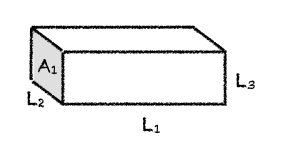
\includegraphics[width=8cm]{fig/Fig1}
\caption{\label{fig:fig1} Bloco retangular.}
\vspace{-0.4cm}
\end{center}
\end{figure}
\begin{num}
\item Determine a área A1 com a incerteza correspondente.
\item Determine o volume desta peça com a incerteza correspondente.
\item Se a precisão necessária para o resultado da área é de 0,5\% podemos considerar este resultado satisfatório?
\end{num}

\item Para determinar a altura de uma cachoeira, algumas pessoas mediram o tempo de queda de pedrinhas que eram soltas, em queda livre, de um mesmo local. Conhecendo o tempo de queda $t$, pode-se calcular a altura $h$ a partir da relação cinemática $h = 1/2 g t^2$ em que $g$ é a aceleração da gravidade. Foi utilizado um cronômetro com precisão de centésimos de segundo e os valores $t_i$ obtidos em 8 medidas estão na seguinte tabela:

\begin{center}
  \begin{tabular}{|>{ \centering\arraybackslash}m{1cm}  |>{ \centering\arraybackslash}m{2cm} |}  \hline
    	& t(s)	 \\ \hline	 	
  1	& 1,30\\ \hline	 
2	&1,09\\ \hline	 
3	&1,03\\ \hline	 
4	&1,27\\ \hline	 
5	&1,18\\ \hline	 
6	&1,31\\ \hline	 
7	&1,24\\ \hline	 
8	&1,15\\ \hline	 
  \end{tabular}
  \end{center}

Considerando $g = (9,784 \pm 0,001)$~m/s$^2$, calcule a altura da cachoeira e a sua incerteza.

\end{num}

